\chapter{Présentation du projet}

%doit contenir la fonction de ce rapport : etat de l'art + previsionnel
%dans le but de réaliser un projet
\section{Présentation}
Dans le cadre de ce projet, nous sommes amené à rédiger un état de la l'art.
Cette première partie, nous permet de synthétiser et sélectionner les 
solutions. Notre objectif étant de détecter la main et les articulations 
de la main d'une personne, afin de modéliser en 3D la main de cette personne, 
dans des plans de caméra global ou rapprocher. Cela doit être réalisable en 
temps réel et à partir d'une caméra nous fournissant une image RGB et une 
image contenant l'information de profondeur de la scène filmée.\\

De plus en plus d'application nécessite des IHM plus précisent et plus 
naturelles. Pour cela, la détection de la main devient de plus en plus 
intéressant pour les simulations. Ce niveau de précision peut être
utile dans des simulations médicales où les mains sont l'outils principales 
de l'utilisateur.\\ % Autres exemples?

%doit contenir l'ensemble des informations sur l'équipe -> sur quoi porte leur recherche
\section{Contexte}
La réalisation de ce projet se fait avec l'équipe 3D SAM\footnote{Modeling 
and Analysis of Static and Dynamic Shapes}. Cette équipe conçoit de 
nouveaux outils et méthodes d'analyse des formes des objets 3D statiques 
et dynamique. Ils travaillent sur l'analyse de formes des objects 3D et la 
modélisation des variations des formes dans des vidéos 3D. Nous démarrons 
ce projet proposé par l'équipe, il ne s'agit pas d'une reprise d'un projet 
déjà entamé. Nous travaillons avec la caméra Kinect2 et l'outils Unity3D 
pour la modélisation et l'animation de la main.

%pourquoi faire ce projet (plus de precision?) + cas concret ou on pourrait l'utiliser (ex : medecine)
\section{Problèmatique}
La Kinect permet déjà de détecter un squelette contenant quinze représentant 
différentes articulation du corps humain. 
%a revoir
D'autre outils permettent de détecter les mains des utilisateurs, cependant leur
champ de vision n'est pas assez important pour diverse application.

%comment réaliser ce projet, avec quoi + résultat attendu
\section{Objectif}
L'objectif de notre projet est d'utiliser la Kinect 2 dans le but de détecter les différentes articulations
de la main et de modéliser celle-ci dans une application Unity.
%TODO ajouter les différentes étape de nos recherches 

\section{Présentation de la Kinect 2}
La Kinect 2 de Microsoft possède une caméra couleur en mode YUV de 1920x1080 pixel.
YUV est une combination particulière d'information pour restituer la couleur, comme RGB ou HSP.
Cette combinaison aussi appelée YCbCr, avec Y la luminance, U/Cb la composante bleu sans luminance et V/Cr la composante rouge sans luminance
En plus de sa caméra, elle possède 3 diffuseur de rayonnement infrarouges qui servent à dessiner une carte de profondeur.
Les autres fonctionnalités ne nous intéresseront pas résoudre notre problèmatique.

On récupère donc de Kinect les données brutes suivantes : 
\begin{itemize}
 \item un flux vidéo couleur en YUV
 \item un flux vidéo d'images de profondeur
\end{itemize}

Ces deux flux peuvent servir à détecter la main (méthodes expliquées dans la partie état de l'art)

Le SDK de la Kinect fournit des informations déjà traitées. 
Par exemple pour notre projet, les jointures du poignet, du centre de la main, du sommet du pouce et du sommet du majeur.

\begin{figure}[!h]
\center
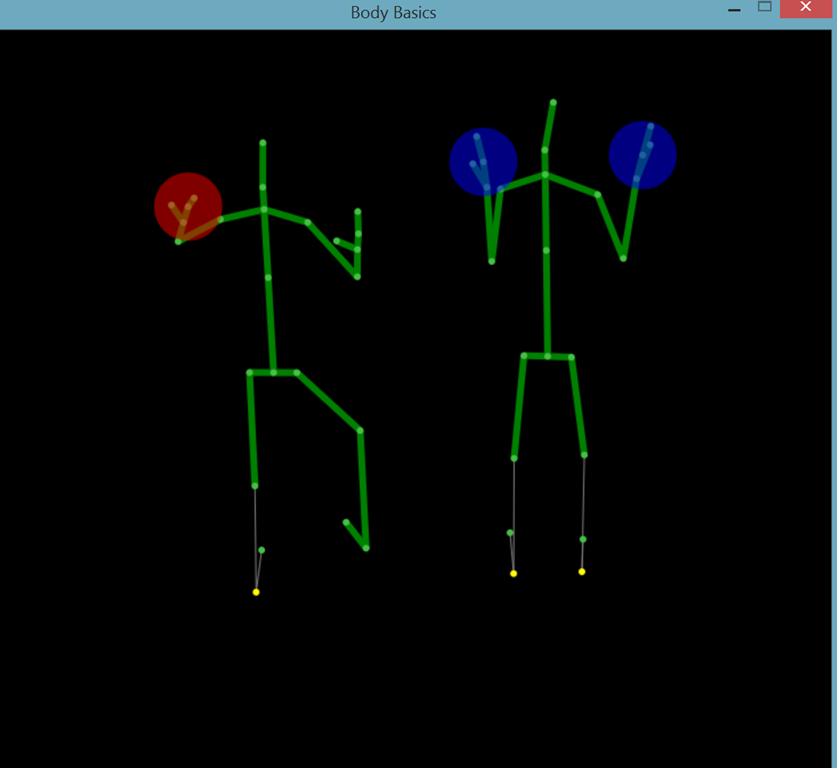
\includegraphics[width=7cm]{images/kinec2_skel.png}
\end{figure}

%présentation du materiel + image materiel
%présentation des données brut
%présentation du sdk + image squelette